\documentclass[a4paper, oneside, 11pt]{article}
%% -> Für längere Arbeiten "report" benutzen.

%% --------------------------------------------------------------------- %%
\usepackage{pdfpages}
\usepackage{ifthen}
\newboolean{english}
%\setboolean{english}{true} %% -> Kommentar entfernen bei englischen Arbeiten

%% --------------------------------------------------------------------- %%

%% -> Einfügen der Definitionen
%% -> Deutsche Anpassung 
\usepackage[T1]{fontenc}
\usepackage[ngerman,english]{babel}
%\usepackage{babelbib}
\usepackage{ifthen}
%% --------------------------------------------------------------------- %%

%% -> Farben einfügen
\usepackage{color}
\usepackage{xcolor}

% -> Definierte Farben
\definecolor{MSBlue}{rgb}{.204,.353,.541} 
\definecolor{trueblue}{rgb}{0.0, 0.45, 0.81}
\definecolor{onyx}{rgb}{0.06, 0.06, 0.06}
\definecolor{mygruen}{rgb}{0.4660, 0.6740, 0.1880}
\definecolor{plotblue}{rgb}{0, 0.4470, 0.7410}
\definecolor{myrot}{rgb}{0.8500, 0.3250, 0.0980}
\definecolor{mygreen}{RGB}{28,172,0} %% Matlab Kommentar
\definecolor{mylilas}{RGB}{170,55,241} %% Matlab String

%% --------------------------------------------------------------------- %%

%% -> Grafiken 
\usepackage{graphicx}
\usepackage{epstopdf}
\usepackage{wallpaper}
\usepackage{float} 
\usepackage[section]%% Verbessert die Platzierung
%% --------------------------------------------------------------------- %%

\usepackage[tmargin=1in,bmargin=1in,lmargin=1.25in,rmargin=1.25in]{geometry}
\setlength{\parindent}{0em}
\setlength{\parskip}{1.5ex plus0.5ex minus0.5ex}
\usepackage{setspace}
\onehalfspacing

\usepackage{pst-all} %% erweiterte Zeichenbefehle

%% -> Schriftart
\usepackage{helvet}
\renewcommand{\familydefault}{phv}

%% -> Layout Überprüfung
\usepackage{layout}
\usepackage{xspace}

%% -> Für Tabellen
\usepackage{array}
\usepackage{booktabs}
\usepackage{dcolumn}
\usepackage{multirow}

%% -> Einrücken von und Abstand zwischen Absätzen
\setlength{\parindent}{0em}
\setlength{\parskip}{1.5ex plus0.5ex minus0.5ex}

%% -> Tabulator Funktion
\newcommand\tab[1][1cm]{\hspace*{#1}}

%% -> Weniger Warnungen wegen überfüllter Boxen
\tolerance = 9999
\sloppy

%% -> Erweiterte Einstellungen der Bildunterschriften bzw. Tabellenunterschriften
\usepackage{caption}
\usepackage{subcaption}
\captionsetup[figure]{labelfont=footnotesize, textfont=footnotesize}
\captionsetup[table]{labelfont=footnotesize, textfont=footnotesize}

%% -> Hyperref
\usepackage[pdftex,bookmarks=true,bookmarksnumbered=true,]{hyperref}

% \usepackage[hidelinks]{hyperref}
%\usepackage[colorlinks=true]{hyperref}
% \hypersetup{
% colorlinks=true,
% linkbordercolor={1 0 0},
% citebordercolor={0 1 0},
% filebordercolor={1 0 1},
% runbordercolor={1 0 1},
% urlbordercolor={0 0 1},
% }

%% -> Quellen
\usepackage[super, square, sort&compress]{natbib}

%%-> Weitere nützliche Pakete
\usepackage{todonotes}
\setlength {\marginparwidth }{2cm}
%% --------------------------------------------------------------------- %%

% -> Für Codes zum einfügen
\usepackage{listings}
%\lstset{numbers=left,numberstyle=\tiny,stepnumber=5,numbersep=5pt}

%% -> Für MATLAB Code
\lstset
{language=Matlab,%
    basicstyle=\scriptsize,
    breaklines=true,%
    captionpos=b,
    frame = single,
    morekeywords={matlab2tikz},
    keywordstyle=\color{blue},%
    morekeywords=[2]{1}, keywordstyle=[2]{\color{black}},
    identifierstyle=\color{black},%
    stringstyle=\color{mylilas},
    commentstyle=\color{mygreen},%
    showstringspaces=false,%
    %numbers=left,%
    %numberstyle={\footnotesize \color{black}},%
    %stepnumber=5, %
    %numbersep=9pt, % 
    emph=[1]{for,end,break},emphstyle=[1]\color{red}, %
    emph=[2]{all}, emphstyle=[2]\color{mylilas},    
}
%% --------------------------------------------------------------------- %%

% -> Kopf und Fußzeile gestallten
\usepackage{fancyhdr}
%\setlength{\headheight}{13.6pt}
\setlength{\footskip}{41pt}
\rhead{} 
\chead{} 
\lhead{}
\renewcommand{\headrulewidth}{0pt}
\lfoot{
\includegraphics[width=\textwidth*1/6]{Definition/DUH-positive.eps}}
\rfoot{\small\thepage}
\cfoot{}
\renewcommand{\footrulewidth}{0pt}
%% --------------------------------------------------------------------- %%

%% -> Matematische Packages
\usepackage{amsmath,amssymb,amsfonts,amstext}
\usepackage{mathtools}
\usepackage{mathrsfs}

%% -> SI-Einheiten
%\usepackage{units}
\usepackage{siunitx}
% \usepackage{physics}
\sisetup{locale = DE,separate-uncertainty}
\sisetup{list-final-separator={ und }}
\sisetup{per-mode=fraction}
\DeclareSIUnit\Pascal{\newton\per\square\metre}
%\sisetup{output-decimal-marker = {.}} %% Für Punkttrennung nur bei englischen Arbeiten erforderlich
%% --------------------------------------------------------------------- %%

%% -> Für die Überschriften
\usepackage{titlesec}
\titleformat{\section}{\LARGE\sffamily\bfseries}{\thesection}{1em}{}
\titleformat{\subsection}{\Large\bfseries\sffamily}{\thesubsection}{1em}{}
\titleformat{\subsubsection}{\large\sffamily\bfseries}{\thesubsubsection}{1em}{}
%% --------------------------------------------------------------------- %%

%% -> Bildnummerierung ist logisch mit Kapitelnummerierung
\numberwithin{figure}{section}
\numberwithin{table}{section}
\numberwithin{equation}{section}
%\numberwithin{equation}{subsection}
%% --------------------------------------------------------------------- %%

%% -> Schaltplan zeichnen und Grafiken und für PGF Plots
\usepackage[european, siunitx]{circuitikz}
\usepackage{tikz}
\usepackage{tikzscale}
\usepackage{pgfplots}
\pgfplotsset{compat=1.4}
\newlength\figH
\newlength\figW
\setlength{\figH}{6cm}
\setlength{\figW}{8cm}
%% --------------------------------------------------------------------- %%

%% -> Für das Formelverzeichnis
\DeclareCaptionType{myequations}[][Formelverzeichnis]
\captionsetup[myequations]{labelformat=empty}
%% --------------------------------------------------------------------- %%

%% -> Für das Symbolverzeichnis
\usepackage[toc, hyperfirst = false, acronym, nonumberlist]{glossaries}
\makeglossaries
%\input{Symbols_Acronym/symbols}
%\input{Symbols_Acronym/acronym}
%% --------------------------------------------------------------------- %%



%% -> Deckblatt ausfüllen 
\def\labtitle{Transient Simulation}
\def\labcode{MECH-M-3-SVE-TSI-ILV}
\def\labname{}
\def\labnum{Berichtnummer}
\def\study{Master Mechatronic \& Smart Technologies}
\def\branch{}
\def\term{3.}
\def\lecturer{Thomas Gadner}
\def\group{MA-MECH-23-BB}
\def\student{Lukas Sieß}

%% --------------------------------------------------------------------- %%
\begin{document}
\newcounter{romanPagenumber}

%% -> Sprache auswählen
\ifthenelse{\boolean{english}}{\selectlanguage{english}}{\selectlanguage{ngerman}}
\selectlanguage{ngerman}
%\selectlanguage{english}

\pagestyle{fancy} % Fußzeile und Kopfzeile einfügen

\pagenumbering{Roman}

%% Deckblatt %%

\thispagestyle{empty}
\sffamily
\ThisTileWallPaper{\paperwidth}{\paperheight}{Deckblatt/MCIHintergrundKPL.pdf}

\vspace*{1cm}
\def\thesis{\ifthenelse{\boolean{english}}{Abschlussbericht}{Aufgaben}}
\textcolor{MSBlue}{\rmfamily\bfseries\Huge\thesis}

\vspace*{0.5cm}
\textbf{\labtitle{} (\labcode)}

\textbf{\labname}

%\ifthenelse{\boolean{english}}{\textbf{Report} }{\textbf{Labor }}\textbf{\labnum}


\vspace*{14cm}

\textcolor{gray}{\study}

% \def\studybranch{\ifthenelse{\boolean{english}}{Study Branch}{Studienzweig}}
% \textcolor{gray}{\studybranch: \branch}

\def\termname{\ifthenelse{\boolean{english}}{semester}{Semester}}
\textcolor{gray}{\term{ }\termname}

\def\lecturername{\ifthenelse{\boolean{english}}{Responsible lecturer}{Lehrveranstaltungsleiter}}
\textcolor{gray}{\lecturername: \lecturer}

\def\groupname{\ifthenelse{\boolean{english}}{Group}{Jahrgang}}
\textcolor{gray}{\groupname: \group}

\def\authorname{\ifthenelse{\boolean{english}}{Author}{Verfasser}}
\textcolor{gray}{\authorname: \student}

\textcolor{gray}{\today}

\newpage % Deckblatt laden

\setcounter{romanPagenumber}{\value{page}}

\tableofcontents%\thispagestyle{empty}   % Inhaltsverzeichnis
\clearpage

\pagestyle{fancy}
\pagenumbering{arabic}
% =============================================================================
\section{Einleitung} \label{sec:einleitung}

Im Rahmen dieser Aufgabenstellung wurden in zwei aufeinander aufbauenden Schritten ein Schaltnetzteil entworfen und die entsprechenden Maßnahmen zur elektromagnetischen Verträglichkeit (EMV) untersucht. Im ersten Teil bestand die Aufgabe darin, eine geregelte Schaltnetzteil-Schaltung in LTspice zu entwickeln, ohne ein Eingangsfilter zu implementieren. Im zweiten Schritt sollte die Schaltung hinsichtlich der leitungsgebundenen Emissionen (differenzielle und Gleichtaktstörungen) analysiert und ein geeignetes Filterdesign entwickelt werden, um die EMV-Tests zu bestehen.

Für die Umsetzung wurde der LTC3639 (Abbildung \ref{fig:LTC3639-1185}), ein Step-Down-Schaltregler von Analog Devices, verwendet. Die Simulationen wurden sowohl ohne als auch mit einem geeigneten Filter durchgeführt.


\begin{figure}[H]
    \centering
    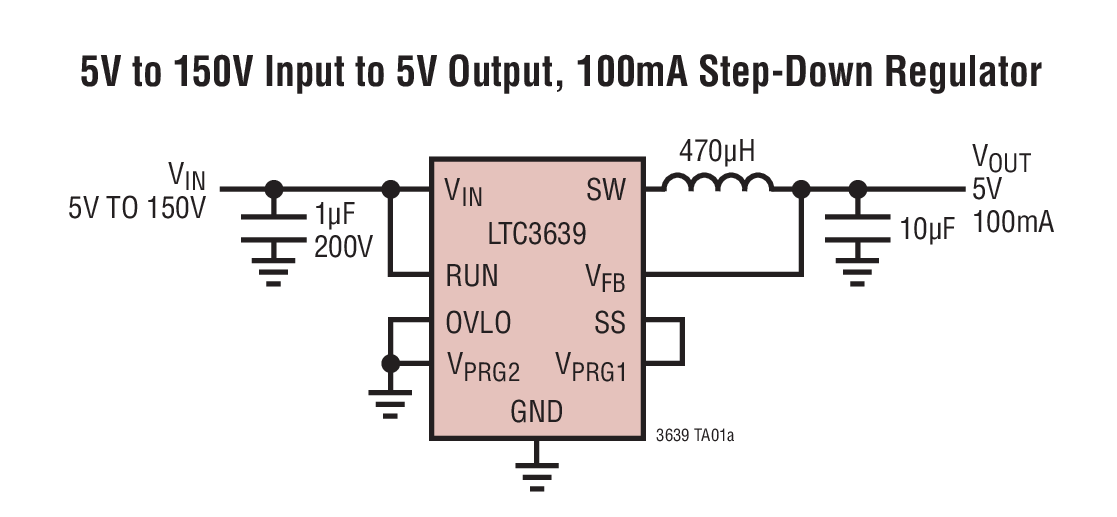
\includegraphics[width=0.8\linewidth]{document/Figure/LTC3639-1185.png}
    \caption{LTC3639-1185}
    \label{fig:LTC3639-1185}
\end{figure}
\newpage
\section{Task 1} \label{sec:Task1}

Die aufgebaute Schaltung mit dem LTC3639 und der zur Verfügung gestellten Eingangsschaltung gemäß Abbildung \ref{fig:LTC3639OhneFilter} wurde unter Berücksichtigung der Herstellerempfehlungen für die Beschaltung des LTC3639 umgesetzt. Alle externen Bauelemente, wie Induktivitäten, Kondensatoren und Widerstände, wurden entsprechend den Vorgaben des Herstellers gewählt, um eine optimale Leistung und Stabilität der Schaltung zu gewährleisten. Diese Auslegung stellt sicher, dass der LTC3639 unter den vorgesehenen Betriebsbedingungen effizient arbeitet.


\begin{figure}[H]
    \centering
    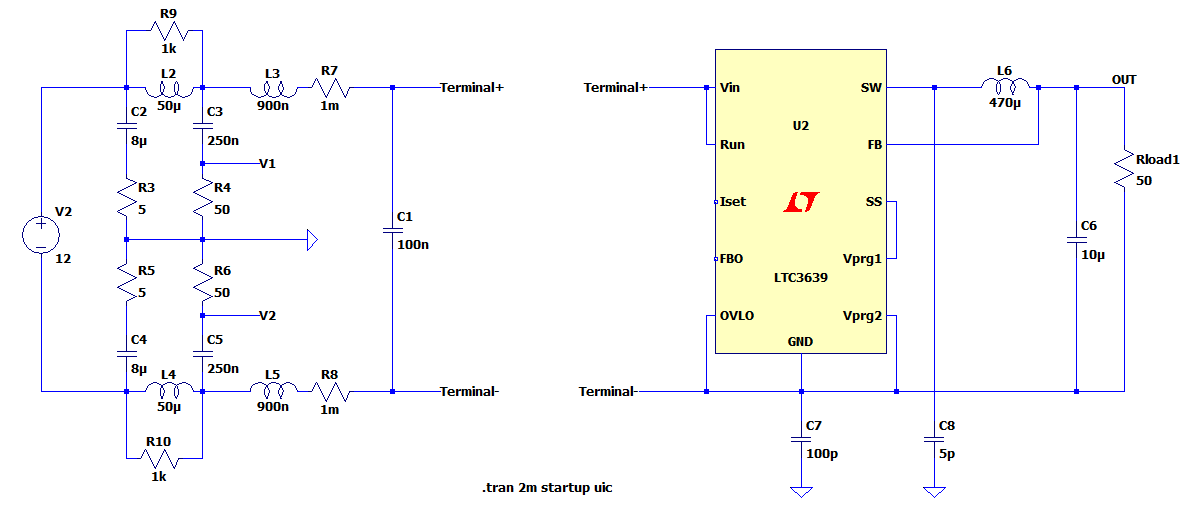
\includegraphics[width=0.8\linewidth]{document/Figure/LTC3639OhneFilter.png}
    \caption{LTC3639 ohne Filter}
    \label{fig:LTC3639OhneFilter}
\end{figure}

\subsection{FFT}

In Abbildung \ref{fig:LTC3639OhneFilterFFT} ist der FFT-Plot der Schaltung ohne Filter zu sehen. Hier zeigt sich, dass die Common-Mode- und Differential-Mode-Interferenzen deutlich über den zulässigen Grenzwerten für die EMV-Zertifizierung liegen. Ohne die Filterung treten hohe Störpegel auf, die die elektromagnetische Verträglichkeit der Schaltung negativ beeinflussen und eine Nicht-Zulassung für die EMV-Zertifizierung zur Folge haben würden.


\begin{figure}[H]
    \centering
    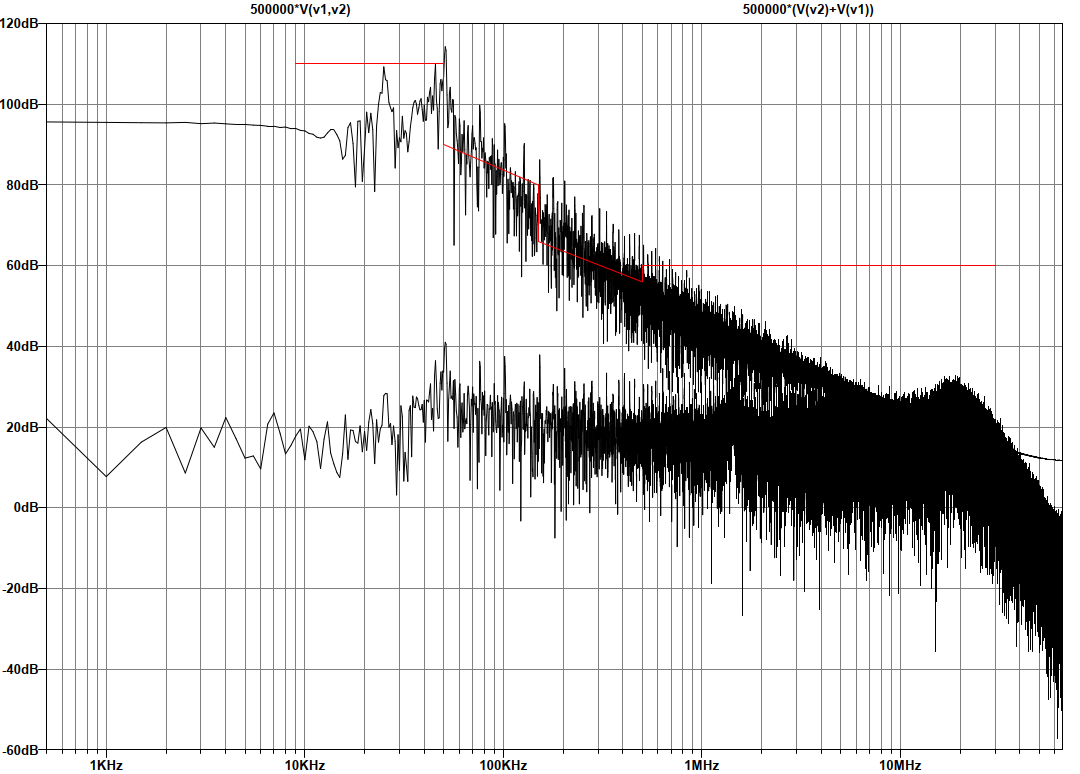
\includegraphics[width=0.8\linewidth]{document/Figure/LTC3639OhneFilterFFT.png}
    \caption{LTC3639 ohne Filter}
    \label{fig:LTC3639OhneFilterFFT}
\end{figure}



\newpage
\section{Task 2} \label{sec:Task2}

Für die Auslegung des Filters wurden die theoretischen Werte der benötigten Bauelemente berechnet, um die Cutoff-Frequenz optimal anzupassen und unerwünschte Störungen zu reduzieren. Ein Filterdesign, das in der Vorlesung besprochen wurde, wurde verwendet, um Resonanzspitzen zu unterdrücken. Eine zusätzliche Dämpfungsstruktur (Damping Branch) wurde integriert, um die Effektivität des Filters weiter zu steigern.

Die Schaltung in abbildung \ref{fig:LTC3639MitFilter} wurde um diesen Filter erweitert, um die EMV-Richtlinien einzuhalten und die leitungsgebundenen Emissionen sowohl im Common-Mode- als auch im Differential-Mode-Bereich zu reduzieren. Abbildung 2 zeigt die erweiterte Schaltung mit dem implementierten Filter, das zur Verbesserung der elektromagnetischen Verträglichkeit beiträgt.

Aufgaben und Auswahl der Komponenten:

\begin{itemize}
    \item \( C_f \) wirkt auf hohe Frequenzen und muss daher ein hochwertiger Kondensator sein, idealerweise ein Keramikkondensator.
    \item \( D_c \) beeinflusst niedrige Frequenzen und kann ein günstiger Elektrolytkondensator sein.
    \item \( C_d \) ist etwa 10- bis 20-mal größer als \( C_f \), um eine effektive Filterwirkung zu gewährleisten.
\end{itemize}

Dieses Design sorgt für eine effektive Dämpfung sowohl von differenziellen als auch von Gleichtaktstörungen und trägt dazu bei, die EMV-Anforderungen zu erfüllen. 

1. Induktivität \(L_f\):
\begin{equation}
    L_f = \frac{\left(\frac{1}{f_g \cdot 2 \pi}\right)^2}{C_f}
    \label{eqn:EffektiveKonvergenzordnung}
\end{equation} 

2. Charakteristischer Widerstand \(R_0\):
\begin{equation}
    R_0 = \sqrt{\frac{L_f}{C_f}}
    \label{eqn:EffektiveKonvergenzordnung}
\end{equation} 

3. Modifizierte Kapazität \(C_d\):
\begin{equation}
    C_d = C_{\text{faktor}} \cdot C_f
    \label{eqn:EffektiveKonvergenzordnung}
\end{equation} 

4. Verhältnis \(n\):
\begin{equation}
    n = \frac{C_d}{C_f}
    \label{eqn:EffektiveKonvergenzordnung}
\end{equation} 

5. Dämpfungswiderstand \(R_d\):
\begin{equation}
    R_d = R_0 \cdot \sqrt{\frac{(2 + n)(4 + 3n)}{(2n)^2(4 + n)}}
    \label{eqn:EffektiveKonvergenzordnung}
\end{equation} 


\begin{figure}[H]
    \centering
    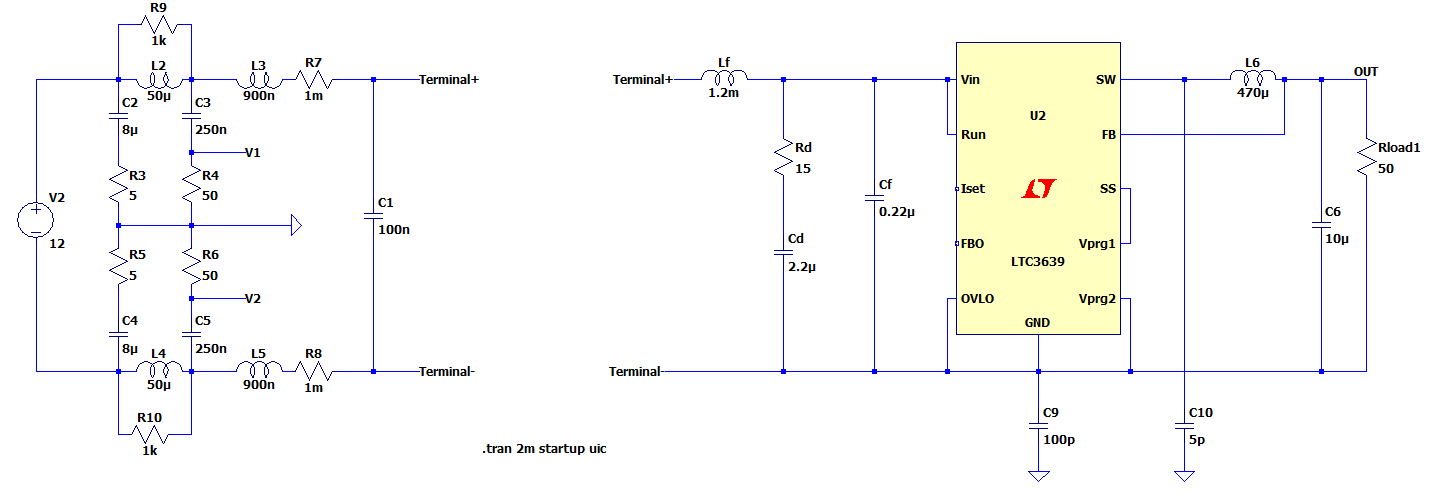
\includegraphics[width=0.8\linewidth]{document/Figure/LTC3639MitFilter.png}
    \caption{LTC3639 mit Filter}
    \label{fig:LTC3639MitFilter}
\end{figure}


\subsection{FFT}

In Abbildung \ref{fig:LTC3639MitFilterFFT} ist der FFT-Plot der Schaltung mit integriertem Filter dargestellt. Es ist erkennbar, dass der Filter seine Funktion erfüllt, indem er sowohl die Common-Mode- als auch die Differential-Mode-Störungen wirksam reduziert und unter die zulässigen Grenzwerte für die EMV-Zertifizierung verschiebt.


\begin{figure}[H]
    \centering
    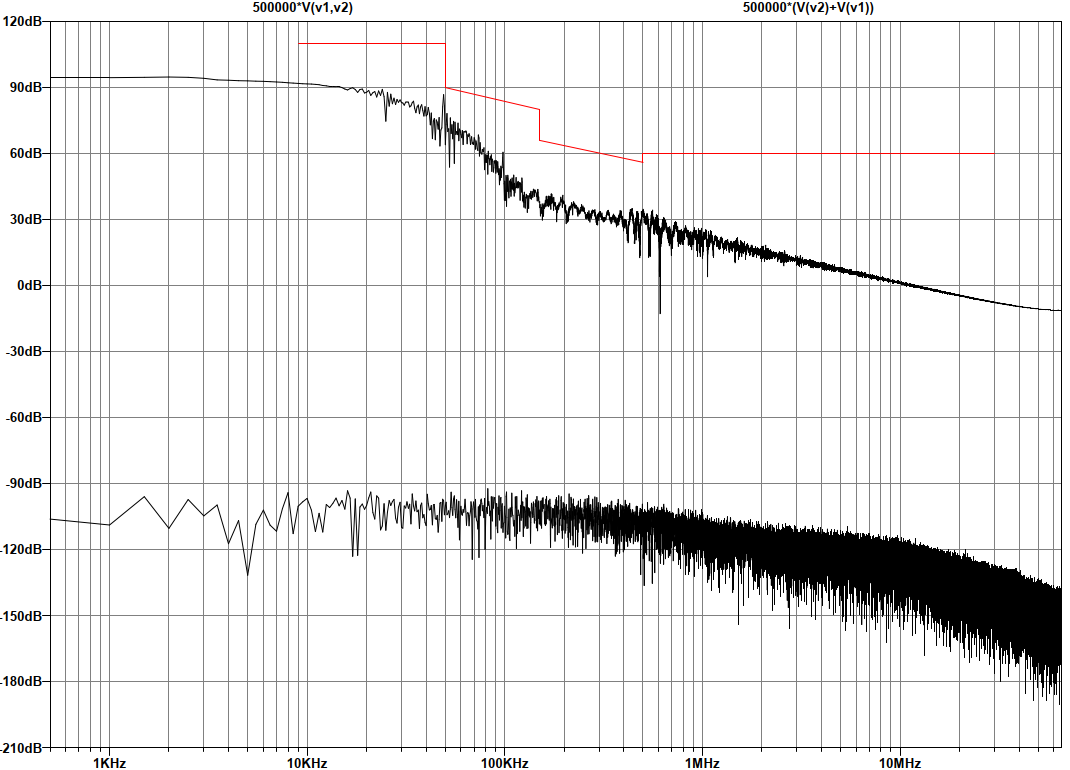
\includegraphics[width=0.8\linewidth]{document/Figure/LTC3639MitFilterFFT.png}
    \caption{FFT LTC3639 mit Filter}
    \label{fig:LTC3639MitFilterFFT}
\end{figure}
\newpage
% =============================================================================

\clearpage

%% -> Verzeichnisse
\pagestyle{fancy}
\pagenumbering{Roman}
\addtocounter{romanPagenumber}{1}
\setcounter{page}{\theromanPagenumber}
%% --------------------------------------------------------------------- %%
\clearpage
%Appendix
\clearpage
\fancyhead[L]{}
\fancyhead[R]{\MakeUppercase{ANHANG}}
\appendix 
\addcontentsline{toc}{section}{ANHANG}
\section{Anhang}\label{app:1} 

\end{document}
